
Onde garantire la qualità di un prodotto software, è indispensabile stilare una suite di test
mirati a verificarne la correttezza. \\
Per questo motivo il gruppo \textit{Bug's Bunny} ha strutturato i test che si trovano a seguire, e ha deciso 
di svolgere l'attività di verifica parallelamente a quella di sviluppo adottando il modello a V\G, 
come definito nelle \NdP\G. \\
I test si suddividono in quattro categorie:

\begin{itemize}
	\item \textbf{Test di unità}:  verificano la correttezza degli elementi atomici del sistema, come ad esempio singoli metodi o classi;
	\item \textbf{Test di integrazione}: verificano che le parti del sistema cooperino correttamente, generalmente controllando il comportamento di gruppi omogenei di unità (che contribuiscono ad un obiettivo comune);
	\item \textbf{Test di sistema}: verificano che l'intero prodotto software funzioni come voluto. Detto in altri termini si verifica che tutti i requisiti obbligatori siano soddisfatti. Vengono svolti alla fine dello sviluppo;
	\item \textbf{Test di accettazione}: effettuati assieme al committente, servono a verificare che il sistema sia conforme alle aspettative. In caso di esito positivo il prodotto viene rilasciato.
\end{itemize}


\subsection{Test di unità}
Questa sezione riporta i test di unità pianificati e/o implementati nei vari componenti dell'applicazione

    \subsubsection{Frontend}
    Qui vengono riportati i test di unità della componente Frontend\G{} dell'applicazione

    {
        \setlength{\freewidth}{\dimexpr\textwidth-10\tabcolsep}
        \renewcommand{\arraystretch}{1.5}
        \centering
        \setlength{\aboverulesep}{0pt}
        \setlength{\belowrulesep}{0pt}
        \rowcolors{2}{Arancione!10}{white}
        \begin{longtable}{C{.3\freewidth} C{.5\freewidth} C{.3\freewidth}}
        \toprule
        \rowcolor{Arancione}
        \textcolor{white}{\textbf{Codice Test}}&
        \textcolor{white}{\textbf{Descrizione}}&
        \textcolor{white}{\textbf{Stato}}\\	
        \toprule
        \endhead

        TUF01.1 & Verificare che ogni classe del file frontend/src/models.ts
                abbia un costruttore che costruisca l'oggetto di quella classe nel modo corretto & Superato \\

        TUF01.2 & Verificare che ogni classe del file frontend/src/models.ts
                supporti nel modo corretto e non ambiguo, come si rischia nel linguaggio di Javascript,
                gli operatori di uguaglianza e di uguaglianza stretta con oggetti della stessa classe & Superato \\

        TUF01.3 & Verificare che il metodo frontend/src/models.ts/Position.distance
                ritorni sempre un numero non negativo & Superato \\

        TUF02.1 & Verificare che frontend/src/utils.ts/capitalizeFirstLetter
                ritorni correttamente una stringa con la prima lettera maiuscola, se presente & Superato \\

        TUF02.2 & Verificare che frontend/src/utils.ts/removeChildren
                rimuova correttamente gli elementi figli da un elemento Html, se presenti & Superato \\

        TUF03.1 & Verificare che il costruttore di LocationPresenter chiami la funzione LocationPresenter.getInfo & Superato \\

        TUF03.2 & Verificare che la funzione LocationPresenter.getInfo inizializzi correttamente un oggetto Info all'interno di LocationPresenter.info 
                formattato nel modo giusto nel caso che le API\G{} siano state caricate in tempo, altrimenti ritorna un errore di timeout & Superato \\

        TUF04.1 & Verificare che il costruttore di ListPresenter chiami la funzione ListPresenter.refresh & Superato \\

        TUF04.2 & Verificare che la funzione ListPresenter.refresh inizializzi correttamente una lista non vuota di Location all'interno di ListPresenter.rankedList, 
                e che queste Location siano valide & Superato \\
        
        TUF05.1 & Verificare che il costruttore di NavPresenter inizializzi correttamente le routes accessibili all'utente in base allo 
                stato di login & Superato \\
        
        TUF06.1 & Verificare che il costruttore di AppPresenter inizializzi correttamente le routes definite all'interno dell'applicazione 
                indipendentemente dallo stato di login & Superato \\

        TUF07.1 & Verificare che il costruttore di HomePresenter inizializzi correttamente la visualizzazione in base alle preferenze 
                dell'utente loggato & Superato \\

        TUF08.1 & Verificare che il costruttore di FollowedPresenter chiami una volta la funzione FollowedPresenter.refresh & Superato \\

        TUF08.2 & Verificare che la funzione FollowedPresenter.refresh modifichi correttamente la lista di profili da visualizzare 
                e che disabiliti correttamente gli input & Superato \\

        TUF08.3 & Verificare che la funzione FollowedPresenter.removeFollowed gestisca correttamente situazioni di successo 
                e di errore e che aggiorni la lista di profili da visualizzare dopo che viene eseguita & Superato \\

        TUF08.4 & Verificare che alla distruzione FollowedPresenter cancelli correttamente i timer ancora in esecuzione 
                e gli errori da esso visualizzati & Superato \\

        TUF09.1 & Verificare che il costruttore di ExplorePresenter chiami una volta la funzione ExplorePresenter.refresh & Superato \\

        TUF09.2 & Verificare che la funzione ExplorePresenter.refresh modifichi correttamente la lista di profili da visualizzare 
                e che disabiliti correttamente gli input & Superato \\

        TUF09.3 & Verificare che la funzione ExplorePresenter.addProfile gestisca correttamente situazioni di successo 
                e di errore e che aggiorni la lista di profili da visualizzare dopo che viene eseguita & Superato \\

        TUF09.4 & Verificare che alla distruzione ExplorePresenter cancelli correttamente i timer ancora in esecuzione 
                e gli errori da esso visualizzati & Superato \\

        TUF10.1 & Verificare che la funzione AddProfilePresenter.search modifichi correttamente il profilo da visualizzare 
                e che disabiliti correttamente gli input & Superato \\

        TUF10.2 & Verificare che la funzione AddProfilePresenter.addProfile gestisca correttamente situazioni di successo 
                e di errore e che rimuova i dati della ricerca precedente dopo che viene eseguita & Superato \\

        TUF10.3 & Verificare che alla distruzione AddProfilePresenter cancelli correttamente i timer ancora in esecuzione 
                e gli errori da esso visualizzati & Superato \\

        TUF11.1 & Verificare che il costruttore di AccountPresenter inizializzi correttamente i dati dell'account da visualizzare & Superato \\

        TUF11.2 & Verificare che AccountPresenter sia responsive ai cambiamenti nei dati dell'account e dello stato di login & Superato \\

        TUF11.3 & Verificare che AccountPresenter.logout effettui il logout locale nel modo corretto 
                e che reindirizzi alla pagina corretta per il logout della sessione di AWS Cognito\G{} & Non implementabile con l'environment `JSDOM' \\

        TUF11.4 & Verificare che AccountPresenter.changePreference gestisca correttamente situazioni di successo 
                e di errore mentre disabilita gli input nel modo corretto & Superato \\

        TUF11.5 & Verificare che alla distruzione AccountPresenter cancelli correttamente i timer ancora in esecuzione 
                e gli errori da esso visualizzati & Superato \\

        TUF12.x & Verificare il corretto funzionamento di MapPresenter & Non Implementato \\

        TUF13.1 & Verificare che locationModel.getInfo ritorni i risultati o gli errori corretti in tutti i casi & Superato \\

        TUF14.1 & Verificare che profilesModel.getFollowed ritorni i risultati o gli errori corretti in tutti i casi & Superato \\

        TUF14.2 & Verificare che profilesModel.removeFollowed ritorni i risultati o gli errori corretti in tutti i casi & Superato \\

        TUF14.3 & Verificare che profilesModel.getMostPopularProfiles ritorni i risultati o gli errori corretti in tutti i casi & Superato \\

        TUF14.4 & Verificare che profilesModel.getProfile ritorni i risultati o gli errori corretti in tutti i casi & Superato \\

        TUF14.5 & Verificare che profilesModel.followProfile ritorni i risultati o gli errori corretti in tutti i casi & Superato \\

        TUF15.1 & Verificare che RequestOptions.getRequestOptions ritorni correttamente le opzioni di ricerca 
                in ogni caso possibile di login o di parametro account & Superato \\

        TUF15.2 & Verificare che RequestOptions.postRequestOptions ritorni correttamente le opzioni di ricerca 
                in ogni caso possibile di login o di parametro account & Superato \\

        TUF16.1 & Verificare che resultsModel aggiorni correttamente il SessionStorage al cambiamento della lista di luoghi & Superato \\

        TUF16.2 & Verificare che resultsModel.getRankedList ritorni i risultati o gli errori corretti in tutti i casi & Superato \\

        TUF16.3 & Verificare che resultsModel.getById trovi correttamente tutti i luoghi presenti nella lista 
                e che ritorni un valore nullo in caso che non sia presente & Superato \\

        TUF17.1 & Verificare che accountModel aggiorni correttamente il SessionStorage al cambiamento dell'account & Superato \\

        TUF17.2 & Verificare che accountModel.createAccount inizializzi correttamente l'account a partire dai token cifrati 
                ritornati dalla pagina gestita di AWS Cognito\G{} & Superato \\

        TUF17.3 & Verificare che accountModel.getAccount ritorni correttamente l'account sia in caso 
                che l'utente sia loggato che non (ritorna null in questo caso) & Superato \\

        TUF17.4 & Verificare che accountModel.cambiaPreferenza ritorni i risultati o gli errori corretti in tutti i casi & Superato \\

        TUF17.5 & Verificare che accountModel.logout effettui correttamente il logout locale, 
                cancellando l'account dalla memoria & Superato \\

        \bottomrule
        \rowcolor{white}
        \caption{Tabella dei test di unità del frontend}
        \end{longtable}
    }
    \subsubsection{Backend}
    I test effettuati nel backend sono stati primariamente incentrati sulla verifica
    delle singole funzionalità atomiche.\\
    Si è raggiunto un buon grado di percentuale di tests passati e una discreta code coverage:
    \begin{figure}[H]
        \centering
        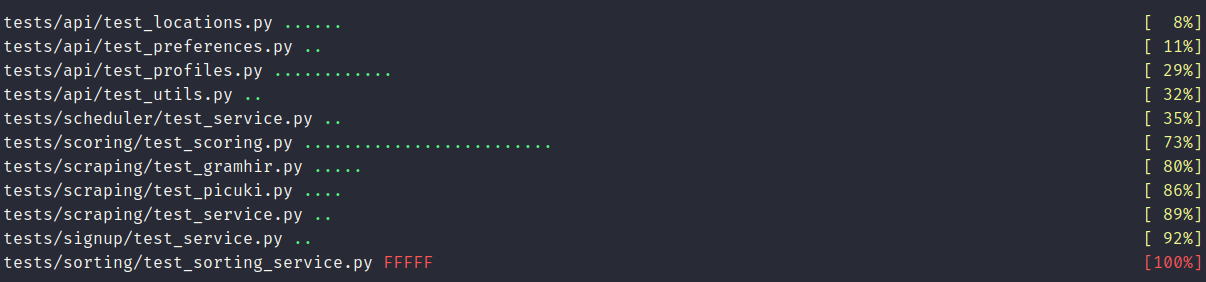
\includegraphics[scale = 0.4]{sezioni/Images/backend_test_passed.png}
        \caption{Percentuale test passati}
    \end{figure}

    \begin{figure}[H]
        \centering
        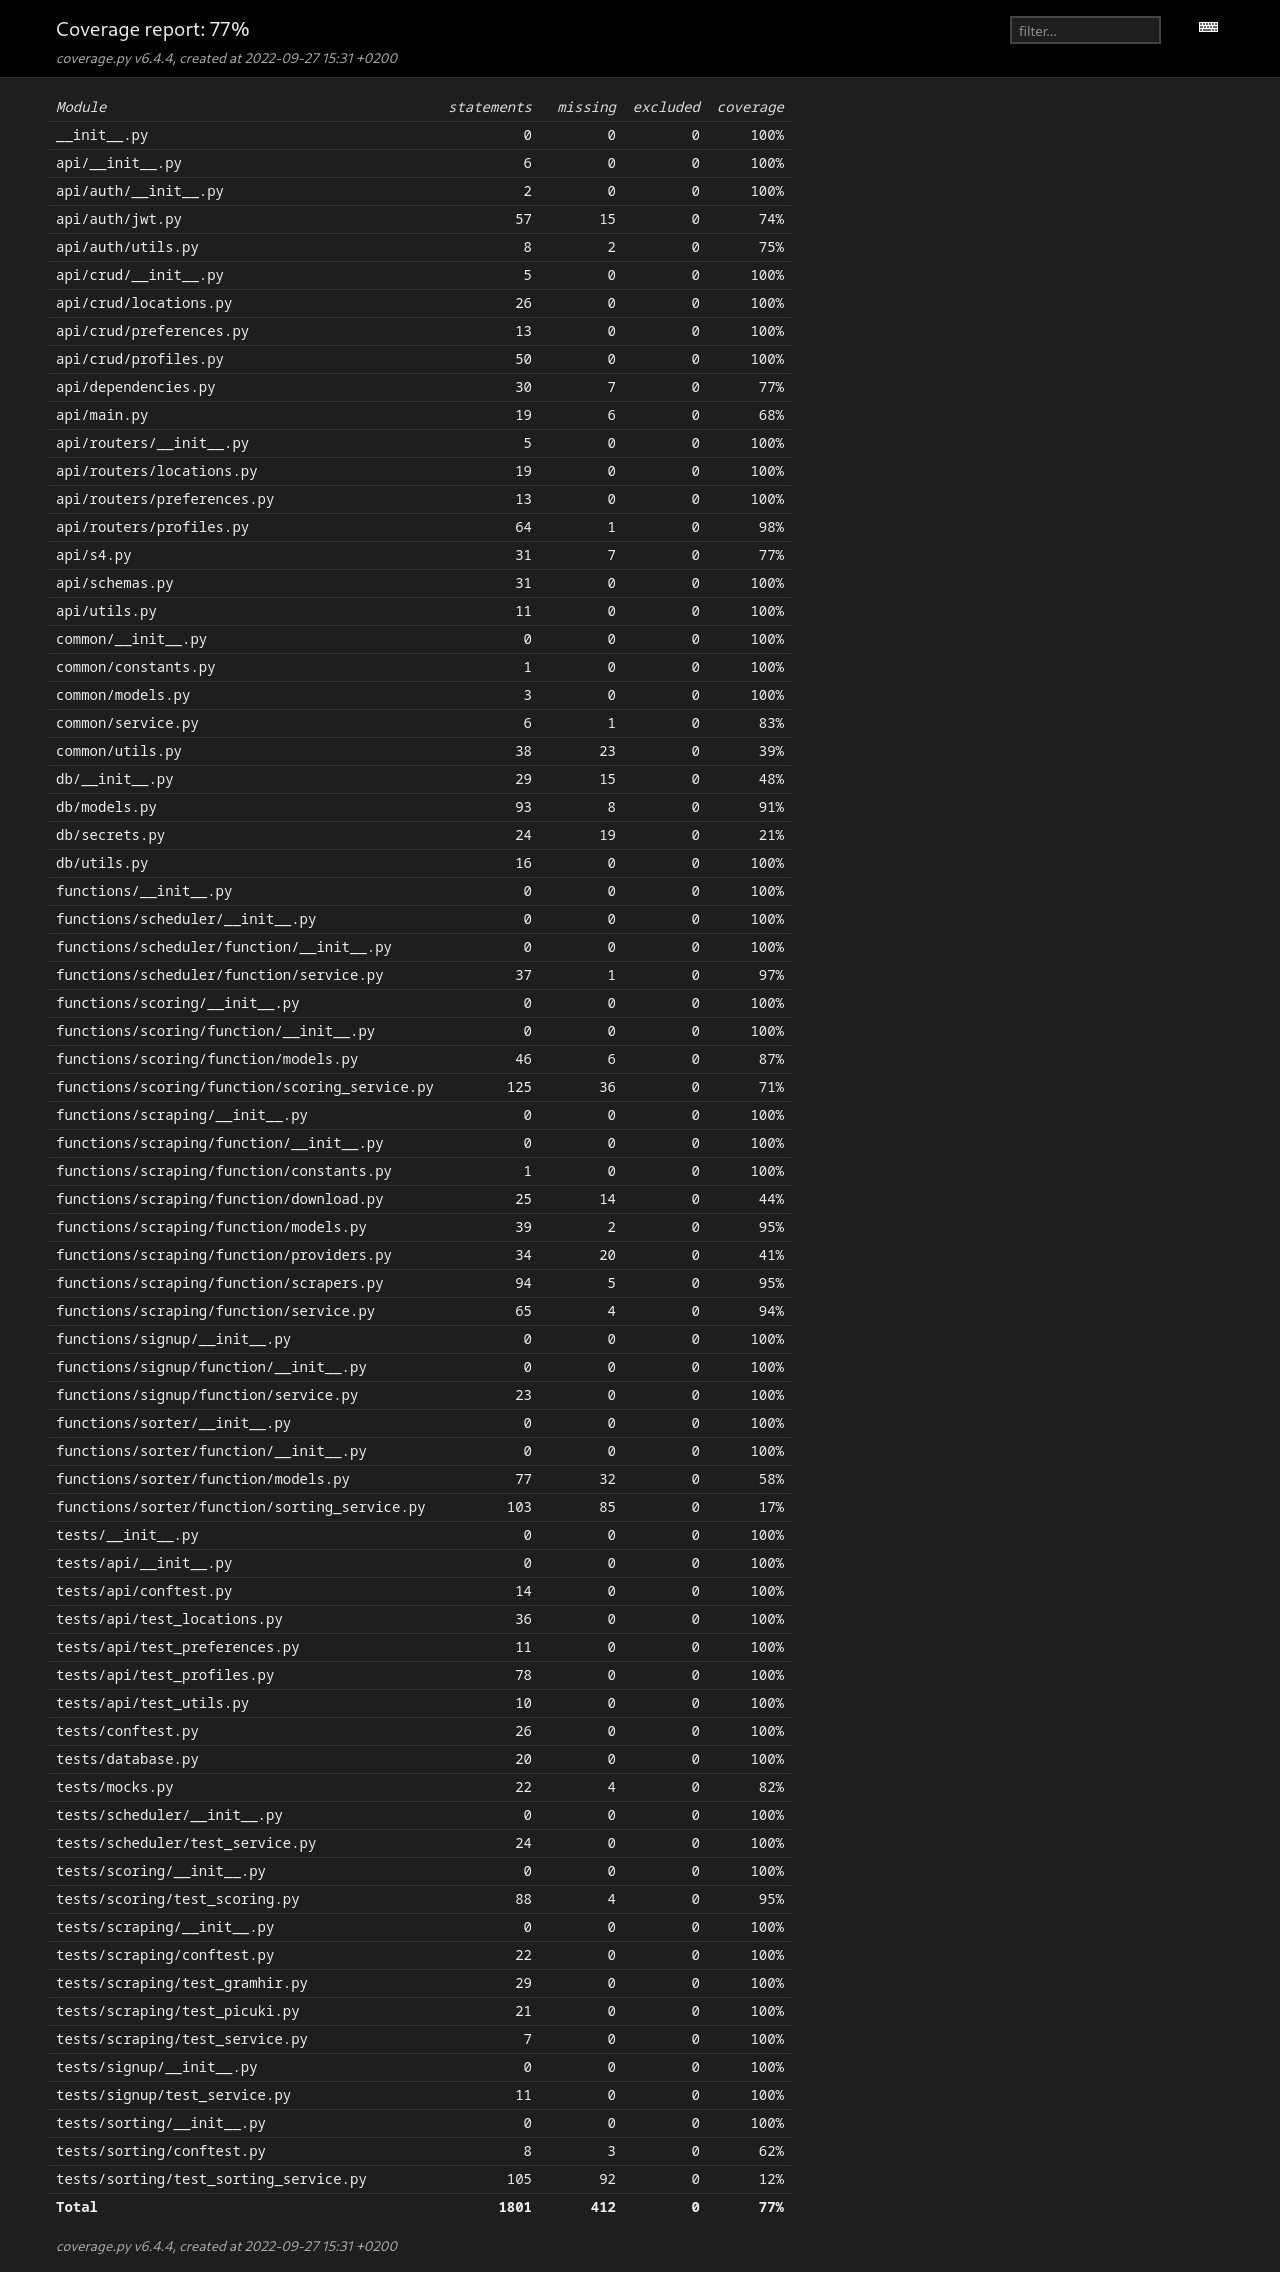
\includegraphics[scale = 0.3]{sezioni/Images/backend_code_coverage.png}
        \caption{Code coverage}
    \end{figure}
    
 
\subsection{Test di integrazione}
    Questa sezione riporta i test di integrazione tra i vari componenti dell'applicazione

    {
        \setlength{\freewidth}{\dimexpr\textwidth-10\tabcolsep}
        \renewcommand{\arraystretch}{1.5}
        \centering
        \setlength{\aboverulesep}{0pt}
        \setlength{\belowrulesep}{0pt}
        \rowcolors{2}{Arancione!10}{white}
        \begin{longtable}{C{.3\freewidth} C{.5\freewidth} C{.3\freewidth}}
        \toprule
        \rowcolor{Arancione}
        \textcolor{white}{\textbf{Codice Test}}&
        \textcolor{white}{\textbf{Descrizione}}&
        \textcolor{white}{\textbf{Stato}}\\	
        \toprule
        \endhead

        TI01 & Verificare che l'integrazione tra la componente Frontend\G{} e la pagina di login/registrazione gestita da Cognito\G{} (e viceversa) 
            sia gestita in modo corretto & Non implementato \\

        TI02 & Verificare che l'integrazione tra le classi in frontend/src/models/ e i relativi endpoint dell'API\G{} backend\G{} siano
            gestiti in modo corretto, gestendo tutte le risposte possibili del backend\G{} & Superato assieme ai TUF dal 13.x al 17.x (test separati e paralleli a questi) \\

        \bottomrule
        \rowcolor{white}
        \caption{Tabella dei test di unità del frontend}
        \end{longtable}
    }

    Una nota sul TI02 è che ogni unit test che testa una funzione che fa una richiesta al server passa automaticamente per un mock server implementato nella cartella dedicata agli integration test `frontend/src/test/integration'
    che fa automaticamente i controlli sulla richiesta inviata dal model utilizzando la specifica OpenApi scaricata dinamicamente all'ultima versione dal server statico del Frontend.

    Controllando il fatto che la richiesta aderisca alla specifica API del backend (e successivamente anche la risposta, garantendo così risposte veritiere nonostante siano `falsificate'), si può testare con molto buona fedeltà
    l'integrazione tra Frontend e Backend tramite l'API. 
    
    Stessa cosa avviene falsificando le Google Maps API, garantendo così un integration testing locale (eccetto il download della specifica API) e un developement server 
    gratuito e veritiero utilizzando quasi lo stesso mock server utilizzato per il testing.

\subsection{Test di accettazione}
Questa sezione  riporta i test di accettazione del prodotto, hanno lo scopo di validare il prodotto.

\subsubsection{Test di accettazione}

{
    \setlength{\freewidth}{\dimexpr\textwidth-10\tabcolsep}
    \renewcommand{\arraystretch}{1.5}
    \centering
    \setlength{\aboverulesep}{0pt}
    \setlength{\belowrulesep}{0pt}
    \rowcolors{2}{Arancione!10}{white}
    \begin{longtable}{C{.1\freewidth} C{.80\freewidth} C{.1\freewidth}}
       \toprule
    \rowcolor{Arancione}
    \textcolor{white}{\textbf{Codice Test}}&
    \textcolor{white}{\textbf{Descrizione}}&
    \textcolor{white}{\textbf{Stato}} \\	
    \toprule
    \endhead

    TA1 & Verificare che l'utente sconosciuto durante la registrazione possa: \begin{enumerate}
        \item inserire la propria mail;
        \item inserire il proprio nome utente;
        \item  inserire la propria password;
        \item visualizzare un messaggio di errore nel caso in cui le informazioni inserite nel campo email siano invalidi;
        \item visualizzare un messaggio di errore nel caso in cui venga inserito un nome utente non valido;
        \item visualizzare un messaggio di errore nel caso in cui venga inserita una password  non valida.
    \end{enumerate}  & N/I \\

    TA2 & Verificare che l'utente non autenticato durante il login possa:\begin{enumerate}
        \item  inserire il proprio nome utente;
        \item   inserire la propria password;
        \item   decidere se memorizzare la sezione;
        \item   visualizzare un messaggio di errore nel caso in cui venga inserito un nome utente non valido;
        \item  visualizzare un messaggio di errore nel caso in cui venga inserita una password  non valida.
    \end{enumerate} & N/I  \\
 
    TA3 & Verificare che l'utente non autenticato con sessione memorizzata durante il login possa:\begin{enumerate}
        \item accedere al sistema;
        \item autenticarsi automaticamente.
    \end{enumerate} & N/I \\

    TA4 & Verificare che l'utente autenticato possa:\begin{enumerate}
        \item selezionare l'azione di logout;
        \item eseguire logout.
    \end{enumerate} & N/I  \\

    TA5 & Verificare che l'utente autenticato possa:\begin{enumerate}
        \item accedere al proprio profilo;
        \item accedere alla pagina di modifica password;
        \item inserire la password attuale;
        \item inserire la nuova password;
        \item confermare la nuova password;
        \item confermare la modifica password;
        \item visualizzare un messaggio di errore nel caso in cui la password sia errata;
        \item visualizzare un messaggio di errore nel caso in cui la nuova password non coincida con la sua ripetizione;
        \item visualizzare un messaggio di errore nel caso in cui la nuova password inserita non sia valida.
    \end{enumerate} & N/I  \\

    TA6 & Verificare che l'utente autenticato possa:\begin{enumerate}
        \item visualizzare la guida in formato mappa se non ha nessun profilo social seguito;
        \item visualizzare la guida in formato lista se non ha nessun profilo social seguito;
        \item visualizzare una mappa personalizzata se ha dei social seguiti;
        \item visualizzare una lista personalizzata se ha dei social seguiti.
    \end{enumerate} & N/I  \\

    TA7 & Verificare che l'utente autenticato possa:\begin{enumerate}
        \item navigare nella sezione dei profili seguiti;
        \item selezionare il pulsante aggiungi profile;
        \item scegliere instagram o tiktok;
        \item Inserire la username di un profilo social da seguire;
        \item confermare e salvare;
        \item visualizzare un messaggio di errore nel caso in cui il profilo inserito non esiste;
        \item visualizzare un messaggio di errore nel caso in cui il profilo inserito è già stato aggiunto ai seguiti.
    \end{enumerate} & N/I  \\

    TA8 & Verificare che l'utente autenticato possa:\begin{enumerate}
        \item navigare nella sezione dei profili seguiti;
        \item selezionare il profilo che vuole rimuovere;
        \item cliccare il pulsante de rimozione.
    \end{enumerate} & N/I  \\

    TA9 & Verificare che l'utente autenticato possa:\begin{enumerate}
        \item navigare nella home;
        \item premere il pulsante per entrare nella pagina di esplorazione;
        \item vedere la lista degli utenti più seguiti sia di instagram che tiktok.
    \end{enumerate} & N/I  \\

    TA10 & Verificare che l'utente autenticato possa:\begin{enumerate}
        \item navigare nella sezione impostazioni;
        \item selezionare la voce vista predefinita;
        \item scegliere la mappa come vista predefinita;
        \item scegliere la lista come vista predefinita.
    \end{enumerate} & N/I \\

\bottomrule
\rowcolor{white}
\caption{Tabella dei test di accettazione di prodotto}
\end{longtable}
} 

\newpage

\subsubsection{Tracciamento di test di accettazione}

{
    \setlength{\freewidth}{\dimexpr\textwidth-10\tabcolsep}
    \renewcommand{\arraystretch}{1.5}
    \centering
    \setlength{\aboverulesep}{0pt}
    \setlength{\belowrulesep}{0pt}
    \rowcolors{2}{Arancione!10}{white}
    \begin{longtable}{C{.27\freewidth} C{.45\freewidth}}
       \toprule
    \rowcolor{Arancione}
    \textcolor{white}{\textbf{Codice Test}}&
    \textcolor{white}{\textbf{Codice caso d'uso}}\\
    \toprule
    \endhead

    TA1 & \begin{itemize}
        \item UC1
        \item UC1.1, UC1.2
        \item UC2
        \item UC3
        \item UC4
    \end{itemize} \\

    
    TA2 & \begin{itemize}
        \item UC5
        \item UC5.1, UC5.2, UC5.3
        \item UC6
        \item UC7
    \end{itemize} \\

    
    TA3 & \begin{itemize}
        \item UC8
    \end{itemize} \\

    
    TA4 & \begin{itemize}
        \item UC9
    \end{itemize} \\

    
    TA5 & \begin{itemize}
        \item UC10
        \item UC10.1, UC10.2, UC10.3, UC10.4
        \item UC11
        \item UC12
        \item UC13
    \end{itemize} \\

    
    TA6 & \begin{itemize}
        \item UC14
        \item UC14.1, UC14.2, UC14.3, UC14.4
    \end{itemize} \\

    
    TA7 & \begin{itemize}
        \item UC15
        \item UC16
        \item UC17
    \end{itemize} \\

    
    TA8 & \begin{itemize}
        \item UC18
    \end{itemize} \\

    
    TA9 & \begin{itemize}
        \item UC19
    \end{itemize} \\

    TA1 & \begin{itemize}
        \item UC20
        \item UC29.1
        \item UC20.2
    \end{itemize} \\

\bottomrule
\rowcolor{white}
\caption{\centering{Tabella del tracciamento di test di accettazione}}
\end{longtable}

}

\subsection{Test di sistema}
\raggedright{I test di sistema dimostrano la totale copertura dei requisiti identificati nel documento \AdR\G.} \\

\subsubsection{Test di sistema}

{
    \setlength{\freewidth}{\dimexpr\textwidth-10\tabcolsep}
    \renewcommand{\arraystretch}{1.5}
    \centering
    \setlength{\aboverulesep}{0pt}
    \setlength{\belowrulesep}{0pt}
    \rowcolors{2}{Arancione!10}{white}
    \begin{longtable}{C{.3\freewidth} C{.5\freewidth} C{.3\freewidth}}
       \toprule
    \rowcolor{Arancione}
    \textcolor{white}{\textbf{Codice Test}}&
    \textcolor{white}{\textbf{Descrizione}}&
    \textcolor{white}{\textbf{Stato}}\\	
    \toprule
    \endhead

    TS1 & Verificare che l'utente possa registrarsi & N/I  \\ 
    TS1.1 & Verificare che l'utente possa inserire un username & N/I  \\
    TS1.2 & Verificare che l'utente possa inserire un username & N/I  \\
    TS1.3 & Verificare che l'utente possa inserire una mail & N/I  \\
    TS1.4 & Verificare che l'utente possa visualizzare un messaggio di errore se ha inserito delle credenziali non valide & N/I  \\
    TS2 & Verificare che l'utente possa autenticarsi ed accedere al proprio account & N/I  \\
    TS2.1 & Verificare che l'utente possa inserire la propria username & N/I  \\
    TS2.2 & Verificare che l'utente possa inserire la propria password & N/I  \\
    TS2.3 & Verificare che l'utente possa visualizzare un messaggio di errore se ha inserito credenziali non validi & N/I  \\
    TS2.4 & Verificare che l'utente possa autenticarsi automaticamente se ha memorizzato la sessione  & N/I  \\
    TS3 & Verificare che l'utente possa effettuare il logout & N/I  \\
    TS4 & Verificare che l'utente possa modificare la propria password & N/I  \\
    TS4.1 & Verificare che l'utente possa inserire la sua password attuale durante l'attività di modifica password & N/I  \\
    TS4.2 & Verificare che l'utente possa inserire la nuova password durante l'attività di modifica password & N/I  \\
    TS4.3 & Verificare che l'utente possa ripetere la nuova password durante l'attività di modifica password & N/I  \\
    TS4.3 & Verificare che l'utente possa ripetere la nuova password durante l'attività di modifica password& N/I  \\
    TS4.4 & Verificare che l'utente possa confermare la modifica della password & N/I  \\
    TS5 & Verificare che l'utente possa visualizzare un messaggio di errore se ha inserito password attuale  non valida & N/I  \\
    TS5.1 & Verificare che l'utente possa visualizzare un messaggio di errore se ha inserito nuova password non valida & N/I  \\
    TS5.2 & Verificare che l'utente possa visualizzare un messaggio di errore se la ripetizione della nuova password e la nuova password non coincidono & N/I  \\
    TS6 & Verificare che l'utente possa visualizzare la guida in formato mappa se non ha nessun profilo social seguito & N/I  \\
    TS6.1 & Verificare che l'utente possa visualizzare la guida in formato lista se non ha nessun profilo social seguito & N/I  \\
    TS6.2 & Verificare che l'utente possa visualizzare la mappa personalizzata se segue dei profili social & N/I  \\
    TS6.3 & Verificare che l'utente possa visualizzare la lista personalizzata se segue dei profili social & N/I  \\
    TS7 & Verificare che l'utente possa aggiungere dei profili social da seguire & N/I  \\
    TS7.1 & Verificare che l'utente possa visualizzare un messaggio di errore nel caso in cui il nome utente che si vuole aggiungere non esiste nel sistema & N/I  \\
    TS7.2 & Verificare che l'utente possa visualizzare un messaggio di errore se l'utente che si vuole seguire è già seguito & N/I  \\
    TS8 & Verificare che l'utente possa rimuovere un profilo social già seguito & N/I  \\
    TS9 & Verificare che l'utente possa esplorare dei profili social più seguiti & N/I  \\
    TS10 & Verificare che l'utente possa impostare  la mappa come vista predefinita & N/I  \\
    TS10.10 & Verificare che l'utente possa impostare  la lista come vista predefinita & N/I  \\
    \bottomrule
    \caption{Tabella dei test di sistema}
\end{longtable}
    
}
\subsubsection{Tracciamento test di sistema}

{
    \setlength{\freewidth}{\dimexpr\textwidth-10\tabcolsep}
    \renewcommand{\arraystretch}{1.5}
    \centering
    \setlength{\aboverulesep}{0pt}
    \setlength{\belowrulesep}{0pt}
    \rowcolors{2}{Arancione!10}{white}
    \begin{longtable}{C{.25\freewidth} C{.25\freewidth}}
       \toprule
    \rowcolor{Arancione}
    \textcolor{white}{\textbf{Codice Test}}&
    \textcolor{white}{\textbf{Codice caso d'uso}}\\
    \toprule
    \endhead

    TS1 & RF1  \\  TS1.1 & RF4  \\   TS1.2 & RF6  \\  TS1.3 & RF4  \\
    TS1.4 & RF4  \\  TS2 & RF2  \\   TS2.1 & RF7  \\  TS2.2 & R8  \\
    TS2.3 & RF8  \\  TS3 & RF8  \\   TS4 & RF9  \\  TS4.1 & RF9  \\
    TS4.2 & RF9  \\  TS4.3 & RF9  \\   TS4.4 & RF9  \\  TS5 & RF10  \\
    TS5.1 & RF10  \\  TS5.2 & RF11  \\   TS6 & RF12  \\  TS6.1 & RF12  \\
    TS6.2 & RF12  \\  TS6.3 & RF12  \\   TS7 & RF15  \\  TS7.1 & RF15  \\
    TS7.2 & RF20  \\  TS8 & RF21  \\      TS9 & RF22  \\    TS10 & RF23  \\
    TS10.1 & RF23  \\
    
    \bottomrule
    \caption{Tabella del tracciamento dei test di sistema}
\end{longtable}
}

\subsection{Struttura dei documenti}
{
    \setlength{\freewidth}{\dimexpr\textwidth-10\tabcolsep}
    \renewcommand{\arraystretch}{1.5}
    \centering
    \setlength{\aboverulesep}{0pt}
    \setlength{\belowrulesep}{0pt}
    \rowcolors{2}{Arancione!10}{white}
    \begin{longtable}{C{.5\freewidth} C{.5\freewidth}}
       \toprule
    \rowcolor{Arancione}
    \textcolor{white}{\textbf{Aspetto}}&
    \textcolor{white}{\textbf{Spiegazione}} \\
    \toprule
    \endhead
    Sezioni fantasma & Le sezioni vuote residue devono essere cancellate \\
    Caption assente &  Tutte le immagini e tabelle devono avere la caption \\
    A capo & Non bisogna spezzare la frasi andando a capo : complica la lettura del documento su \textit{Github}\G\\
    Documento spezzato & Ogni documento deve essere spezzato su più file ".tex", uno per sezione \\
    Ordine alfabetico & I nomi devono essere scritti in ordine alfabetico \\
    
    \bottomrule
    \caption{Tabella riguardo la struttura dei documenti}
\end{longtable}    
    
}
\subsection{Errori ortografici di lingua italiana e di forma}
{
    \setlength{\freewidth}{\dimexpr\textwidth-10\tabcolsep}
    \renewcommand{\arraystretch}{1.5}
    \centering
    \setlength{\aboverulesep}{0pt}
    \setlength{\belowrulesep}{0pt}
    \rowcolors{2}{Arancione!10}{white}
    \begin{longtable}{C{.5\freewidth} C{.5\freewidth}}
       \toprule
    \rowcolor{Arancione}
    \textcolor{white}{\textbf{Aspetto}}&
    \textcolor{white}{\textbf{Spiegazione}}\\
    \toprule
    \endhead

    Errori di battitura & Sono spesso presenti errori di battitura o di distrazione \\
    Discordanza soggetto-verbo & La coniugazione verbale non è coerente con il soggetto \\
    Accenti invertiti & Invertire l'accento acuto con il grave o viceversa \\
    D eufonica & La d eufonica deve essere usata esclusivamente se la vocale della parola successiva è la stessa o in forma quali “ad esempio” e “ ad hoc” \\
    Forma di verbi & Il presente indicativo è da preferire \\
    Forme non concise & Forme come “l'obiettivo è quello di [...]” sono da evitare preferendo versioni concise come "l'obiettivo è [...]”\\
    Forme impersonali & Forme come “ si è deciso di ….” sono da evitare: il soggetto deve essere esplicito \\  
    
    \bottomrule
    \caption{Tabella riguardo gli errori ortografici}
\end{longtable}
}

\newpage

\subsection{Non conformità con le norme di progetto}
{
    \setlength{\freewidth}{\dimexpr\textwidth-10\tabcolsep}
    \renewcommand{\arraystretch}{1.5}
    \centering
    \setlength{\aboverulesep}{0pt}
    \setlength{\belowrulesep}{0pt}
    \rowcolors{2}{Arancione!10}{white}
    \begin{longtable}{C{.5\freewidth} C{.5\freewidth}}
       \toprule
    \rowcolor{Arancione}
    \textcolor{white}{\textbf{Aspetto}}&
    \textcolor{white}{\textbf{Spiegazione}} \\
    \toprule
    \endhead
    Punteggiatura scorretta negli elenchi & Ogni voce di un elenco deve terminare con “;” , a eccezione dell'ultima che termina con “.” \\
    Grassetto negli elenchi & Gli elenchi puntati nella forma “termine: testo” devono avere il termine in grassetto, ma non i “:” \\
    Maiuscolo negli titoli & La maiuscola deve essere usata solo per la prima lettere ed evitata ove non necessaria \\
    Maiuscolo nei elenchi & Le iniziali delle singole voci degli elenchi puntati o numerati vanno in maiuscolo, a meno che la frase che lo precede non finisca con un punto \\
    Ruoli in minuscolo & I ruoli rivestiti nel corso del progetto devono essere in minuscolo \\
    Versione del documento mancante & Quando si riferisce ad un documento va valutato se ci si sta riferendo a una versione in particolare, in quel caso, riportare insieme al nome anche il numero di versione di cui si fa riferimento\\
    
    \bottomrule
    \rowcolor{white}
    \caption{Tabella delle non conformità con le NdP}
\end{longtable}
}
\subsection{Analisi dei requisiti}
{
    \setlength{\freewidth}{\dimexpr\textwidth-10\tabcolsep}
    \renewcommand{\arraystretch}{1.5}
    \centering
    \setlength{\aboverulesep}{0pt}
    \setlength{\belowrulesep}{0pt}
    \rowcolors{2}{Arancione!10}{white}
    \begin{longtable}{C{.5\freewidth} C{.5\freewidth}}
       \toprule
    \rowcolor{Arancione}
    \textcolor{white}{\textbf{Aspetto}}&
    \textcolor{white}{\textbf{Spiegazione}}\\
    \toprule
    \endhead

    Tracciamento UC-R & Ogni caso d'uso deve essere associato a uno o più requisiti \\
    Requisiti & I requisiti devono essere scritti nella forma “[soggetto]” deve/devono [verbo/all'infinito]  \\
    Numerazione UC & La numerazione dei casi d'usi di errore deve appartenere allo stesso livello del caso di successo, che estendono.\\
    UML degli UC & Le estensioni di un caso d'uso vanno nello stesso diagramma UML\G{} del caso d'uso\G{} stesso \\
    
    \bottomrule
    \rowcolor{white}
    \caption{Tabella riguardo l'analisi dei requisiti}
\end{longtable}
    
}
